
% !TeX spellcheck = de_DE
\documentclass{article}

\usepackage[ngerman]{babel}
\usepackage{graphicx}
\usepackage{float}
\usepackage{booktabs}
\usepackage{lscape}
\usepackage{longtable}

\graphicspath{ {./images/} }
\setlength\parindent{0pt}

\makeatletter
\newcommand{\sectionauthor}[1]{
	{\parindent 0em \large \scshape Autor: #1 \par \nobreak \vspace*{1em}}
	\@afterheading
}
\newcommand{\specification}[3]{
	{\parindent 0.5em \hangindent 3em \hypertarget{spec:#1:#2}{\textbf{/#1#2/}} #3 \par \nobreak \vspace*{0.5em}}
}
\makeatother

\title{Bibliotheksanwendung - Feinspezifikation}
\date{\today\\v1.1}
\author{
	Ivan Charviakou\\
	León Liehr\\
	Mohamad Najjar\\
	Jonas Picker\\
	Sergei Pravdin
}

\begin{document}

%--Titel----------------------------------------------------------------------------------------------------------------------------------------------------------------------------------
\maketitle
\begin{figure}[H]
	\centering
	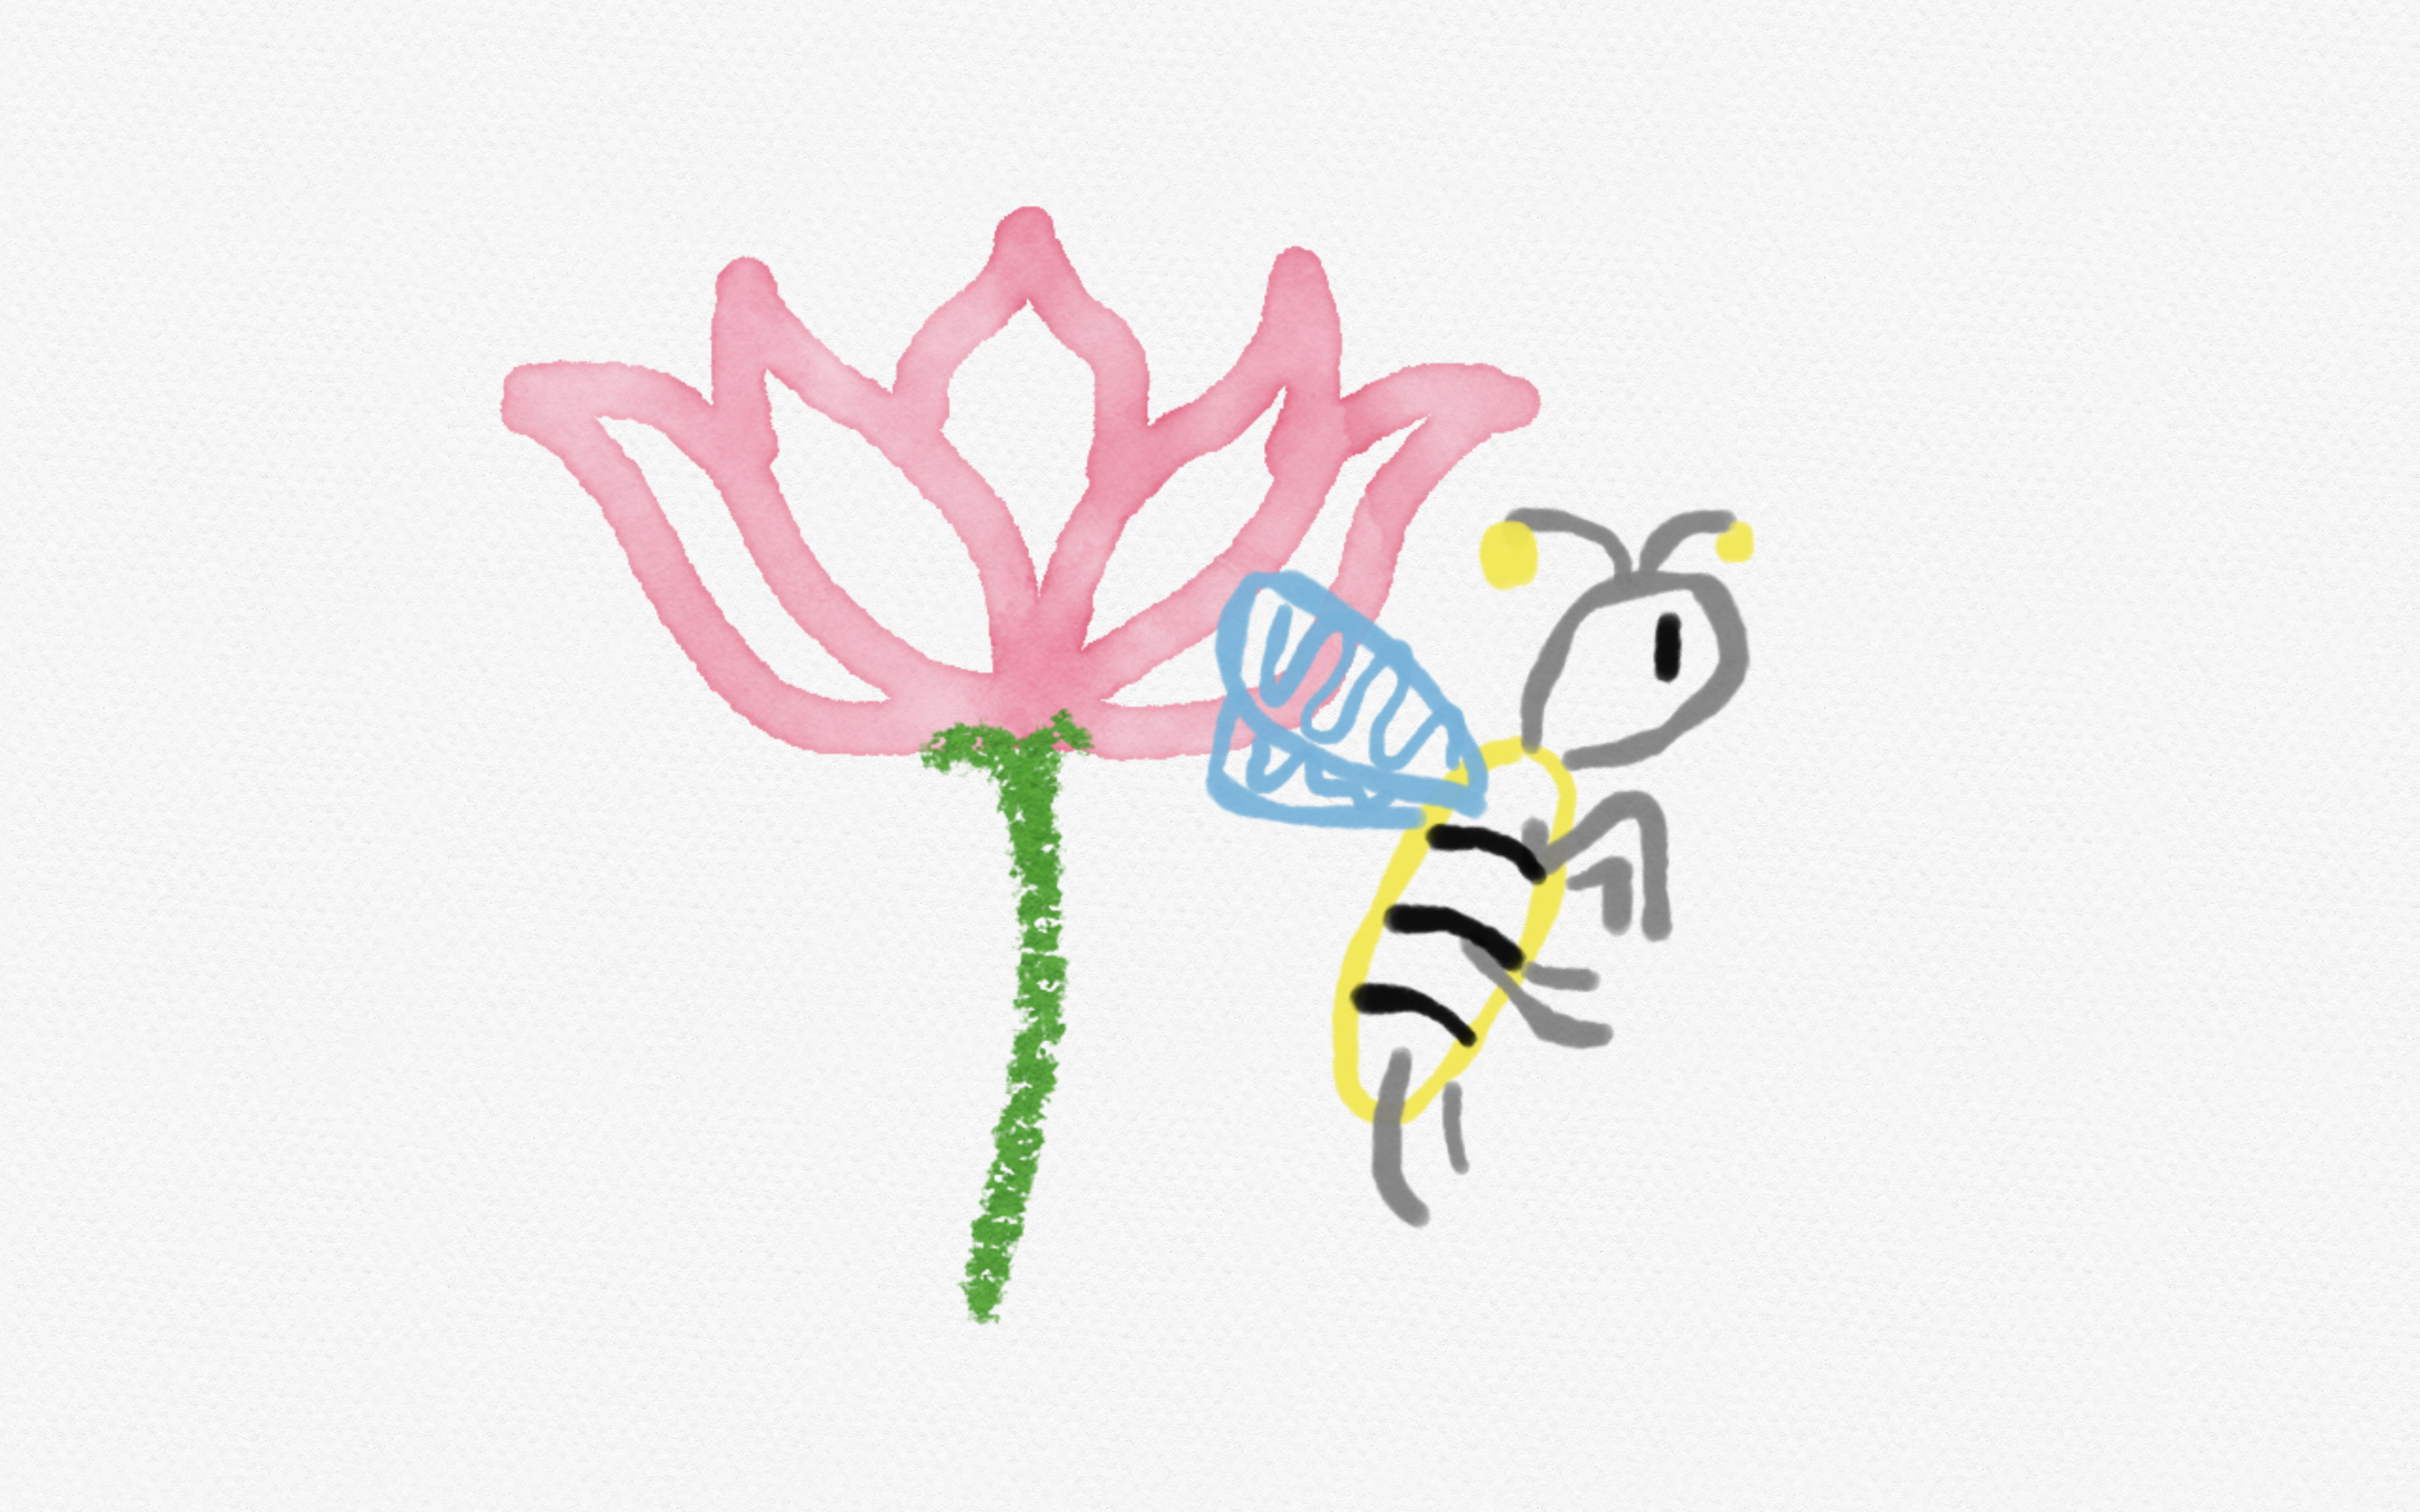
\includegraphics[width = 30em]{Logo}
\end{figure}
\newpage
\tableofcontents
\newpage

%--Einleitung--------------------------------------------------------------------------------------------------------------------------------------------------------------------------
\section{Einleitung}
\sectionauthor{Toad}
Cool text

%--Spezifikation----------------------------------------------------------------------------------------------------------------------------------------------------------------------
\section{Änderungen gegenüber der Spezifikation}
\sectionauthor{Mario}
Cool text

\subsection{Geänderte Views}
Cool list

\subsection{Paketstruktur und verwendete Klassen}
Cool list

\subsection{Datenbankschema}
Cool list

%--Implementierungsplan----------------------------------------------------------------------------------------------------------------------------------------------------------
\section{Änderungen gegenüber dem Implementierungsplan}
\sectionauthor{Luigi}
Cool text

\subsection{Milestone 1}
Cool table

\subsection{Milestone 2}
Cool table

\subsection{Milestone 3}
Cool table

\subsection{Allgemeine Schwierigkeiten}
Cool text

%--Metriken----------------------------------------------------------------------------------------------------------------------------------------------------------------------------
\section{Code-Metriken}
\sectionauthor{Yoshi}
Cool text

%--Reference--------------------------------------------------------------------------------------------------------------------------------------------------------------------------
\section{Reference}
\sectionauthor{Wario}
Cool text

\subsection{Nice looking table}
\begin{longtable}{@{}lllll@{}}
\toprule
\textbf{Header 1} & \textbf{Header 2} & \textbf{Header 3} & \textbf{Header 4} & \textbf{Header 5} \\* \midrule
\endfirsthead
%
\endhead
%
Text 1            & Text 2            & Text 3            & Text 4            & Text 5            \\
Text 1            & Text 2            & Text 3            & Text 4            & Text 5            \\* \bottomrule
\end{longtable}

\subsection{Nice looking landscape-table}
\begin{landscape}
\begin{longtable}{@{}lllll@{}}
\toprule
\textbf{Header 1} & \textbf{Header 2} & \textbf{Header 3} & \textbf{Header 4} & \textbf{Header 5} \\* \midrule
\endfirsthead
%
\endhead
%
Text 1            & Text 2            & Text 3            & Text 4            & Text 5            \\
Text 1            & Text 2            & Text 3            & Text 4            & Text 5            \\* \bottomrule
\end{longtable}
\end{landscape}

\end{document}
